
% -*- mode: latex; coding: latin-1-unix -*- %


\subsection{Circuit Hamiltonien}

\begin{frame}
\frametitle{Circuit Hamiltonien}
\begin{block}{Rappel du probl\`eme}
  \begin{itemize}
  \item Un graphe G,
  \item Est-ce qu'il existe un circuit qui passe une seule fois par
    tous les sommets de G ?
  \end{itemize}
\end{block}
\end{frame}

\begin{frame}
\frametitle{Circuit Hamiltonien}
\begin{block}{R\'eduction vers SAT}
  \begin{itemize}
  \item Un graphe non orient\'e G
  \item Soit \textit{$x_{ij}$} la variable bool\'eenne qui est \`a
    vraie si le sommet \textit{i} se trouve \`a la j-i\`eme position
  \item Soit \textit{n} le nombre de sommets de G : \textit{n*n}
    variables bool\'eennes.
  \end{itemize}
\end{block}
\end{frame}

\begin{frame}
\frametitle{Circuit Hamiltonien}
\begin{block}{Cinq r\`egles de r\'eduction}
  \begin{itemize}
  \item 1) $\forall j \in V(G), (x_{1j} \vee x_{2j} \vee \ldots \vee
    x_{nj})$
  \item 2) $\forall i$ avec $1 <= i <= n$, $(x_{i1} \vee x_{i2} \vee
    \ldots \vee x_{in})$
  \item 3) $\forall i, 1 <= i <= n, \forall {j, k} \in V(G)$, $j \ne
    k$, $(\neg x_{ij} \vee \neg x_{ik})$
  \item 4) $\forall i, 1 <= i <= n, \forall {j, k} \in V(G), {j,k}
    \notin E(G)$, $(\neg x_{ij} \vee \neg x_{i+1,k})$
  \item 5) $\forall j,k \in V(G)$, ${j,k} \notin E(G)$, $(\neg x_{1j}
    \vee \neg x_{nk})$
  \end{itemize}
\end{block}
\end{frame}

\begin{frame}
\frametitle{Circuit Hamiltonien}
\begin{block}{Variables bool\'eennes}
  \begin{itemize}
  \item Sommet 1 : variables situ\'ees dans [ 1 ; n]
  \item ...
  \item Sommet k : variables situ\'ees dans [ (k+1)*n+1 ; k*n ]
  \end{itemize}
\end{block}
\end{frame}

\subsection{Exemples}

\begin{frame}
\frametitle{Exemples}
\begin{block}{Instance positive}
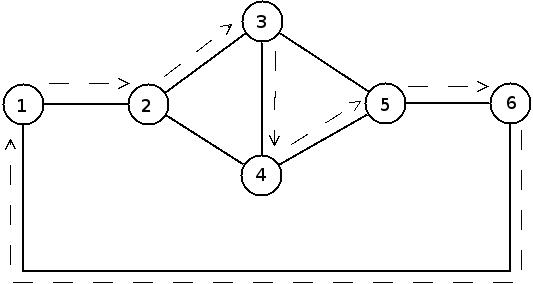
\includegraphics[scale=0.3]{positif.jpeg}
\end{block}
\begin{block}{R\'eponses possibles de SAT}
  \begin{itemize}
  \item R\'eponse : 1 8 15 22 29 36
    \begin{itemize}
    \item (1 2 3 4 5 6)
    \end{itemize}
  \end{itemize}
 \begin{itemize}
  \item R\'eponse : 3 8 13 24 29 34
    \begin{itemize}
    \item (3 2 1 6 5 4)
    \end{itemize}
  \end{itemize}
\end{block}
\end{frame}

\begin{frame}
\frametitle{Exemples}
\begin{block}{Instance n\'egative}
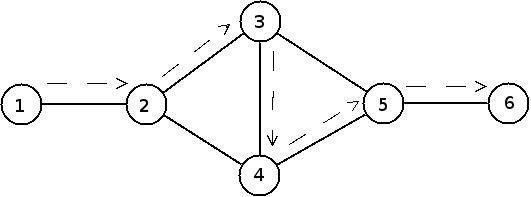
\includegraphics[scale=0.3]{negatif.jpeg}
\end{block}
\begin{block}{R\'eponse de SAT}
  \begin{itemize}
  \item UNSATISFIABLE
  \item Il n'existe pas de circuit hamiltonien pour cete instance.
  \end{itemize}
\end{block}
\end{frame}